%%%%%%%%%%%%%%%%%%%%%%%%%%%%%%%%%%%%%%%%%%%%%%%%%%%%%%%%%%%%%%%%%%%%%%%%%%%%%%%%
%2345678901234567890123456789012345678901234567890123456789012345678901234567890
%        1         2         3         4         5         6         7         8
% THESIS CONCLUSIONS
% \def\baselinestretch{1}
\chapter{Conclusions and future work}
\label{chap:conclusions}
\ifpdf
    \graphicspath{{Conclusions/Figures/PNG/}{Conclusions/Figures/PDF/}{Conclusions/Figures/}}
\else
    \graphicspath{{Conclusions/Figures/EPS/}{Conclusions/Figures/}}
\fi
% \def\baselinestretch{1.0}

% quote
\section{First experiment conclusion}

In the configuration with ADR the ED did not change from SF7. This is problably because 
we were moving and we didn't get 20 uplinks a low maximun SNR to increase the SF. We din't 
get either 64 uplinks without a confirmation as our maximun packet loss between two uplinks 
is 35. (All this is expalined in \ref{chap4:exp1}). In this case the ADR configuration was 
pointless as the end node wasn't able to change the parameters like the SF or the power
to obtain the optimal data transmission. As we got always an spreading factor of 7, the performance 
during the experiment with this configuration is worse compared with the one we selected with SF10 
and a fixed Tx power of 14dBm as you can see in \ref{tab:packet_loss_exp1}. The reason why in 
\ref{tab:RSSI_SNR_exp1}
the values of SNR and RSSI are lower in the case of ADR is because the other configuration 
is able of detecting 
signal in worse situationsas we can see in \\
Thanks to the performance of this experiment we were able to extract 
valuable information releted with the signal received depending on the landscape of the city. 
We distinguish two zones, the area of "vicolis" and the port area:
"Vicoli" is an italian word used in the city of Genova for narrow streets. The historic center of Genova 
is plenty of them making the data transmission almost impossible unless the ED
is close to the gateway (around 100m but it depends if you have direct vision). Next to this zone is the 
area of "porto-antico" which is a much more open-space area where the comunnications reach much longer distances.
The results and graphics shows that the port area showed in the figure (link) is much more 
suitable for a LoRa comunnication rather than the area of the "vicolis".

\section{Second experiment conclusion}
For this second experiment the objective was to further expand on the results that we obtained on the previous one, where we concluded that the packet loss increased exponentially when the device was on a highly building dense area.
After receiving the packets with their locations, we separated, as in figure \vref{chap:conc-div}the map into two regions:
\begin{itemize}
    \item  The lower area, where the conditions resembled the ones in free space
    \item  the upper area where dense buildings can interfere with the signal
\end{itemize}

\begin{figure}[htpb]
\centering    
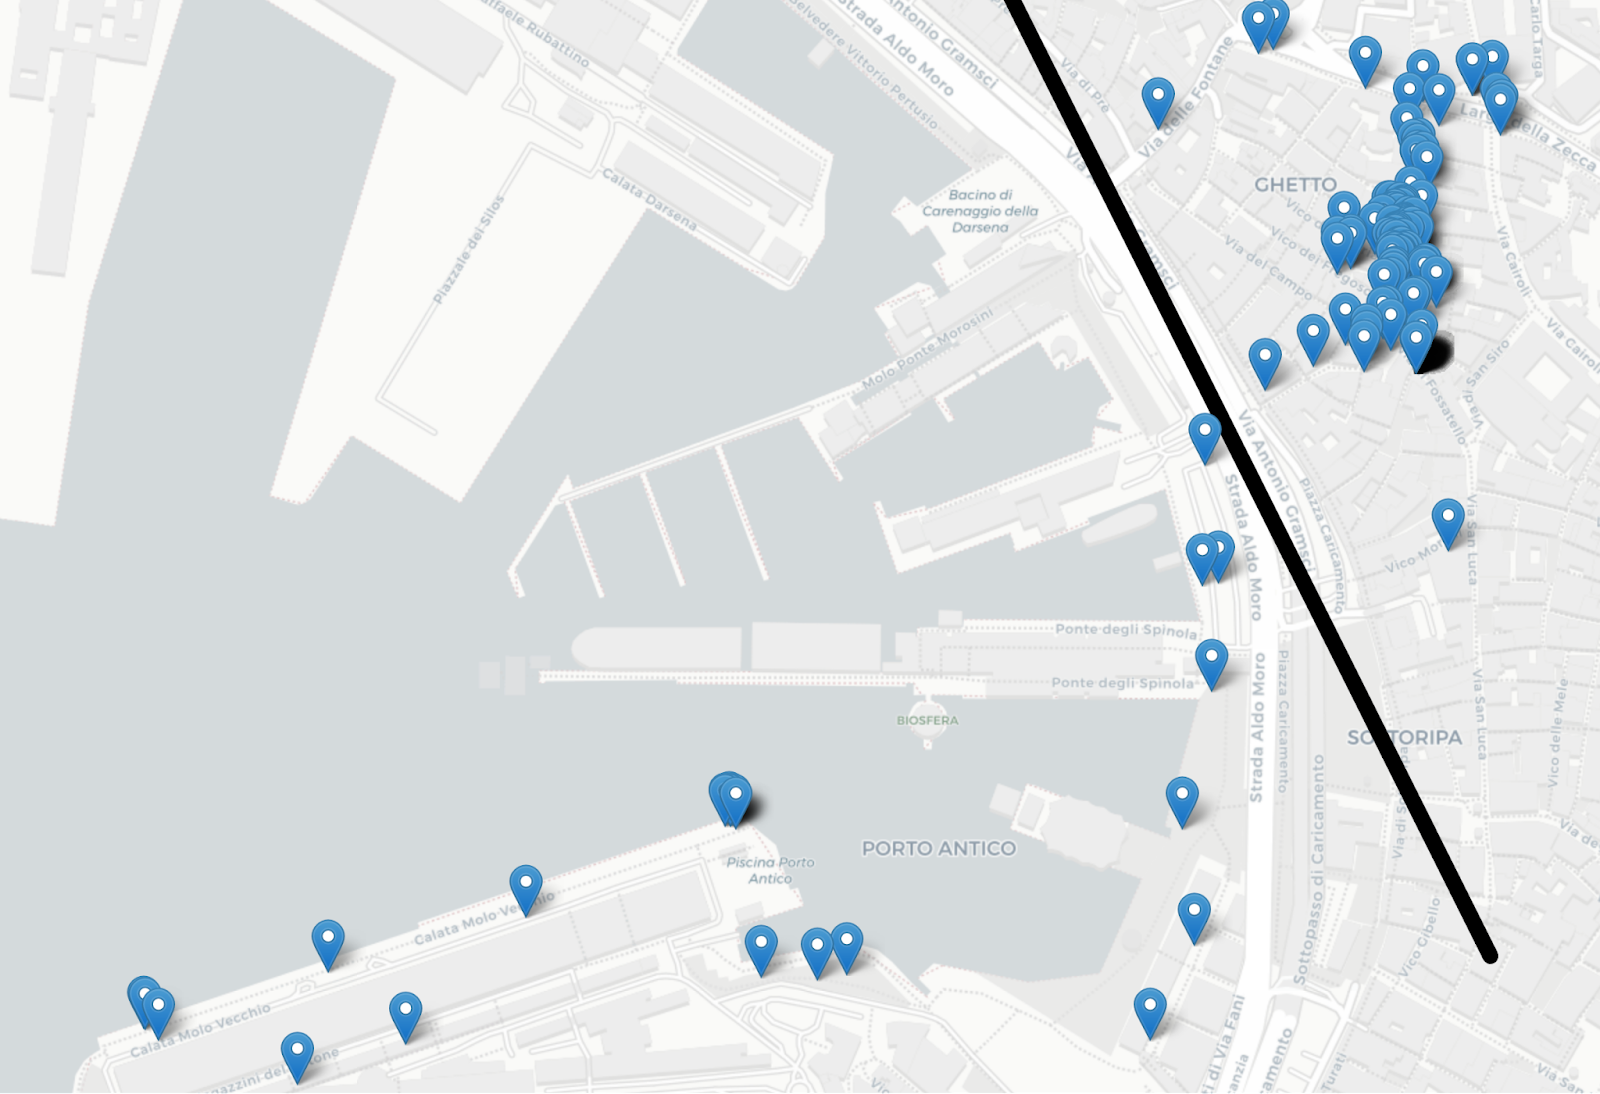
\includegraphics[width=\linewidth]{dividedGenova.png}
\caption{Separation line used}
\label{chap:conc-div}
\end{figure}

This information also allowed us to extract the path followed and know if there had been any losses between the points received.
With that information the map on figure \vref{chap:conc-colpath} map was created:

\begin{figure}[htpb]
\centering    
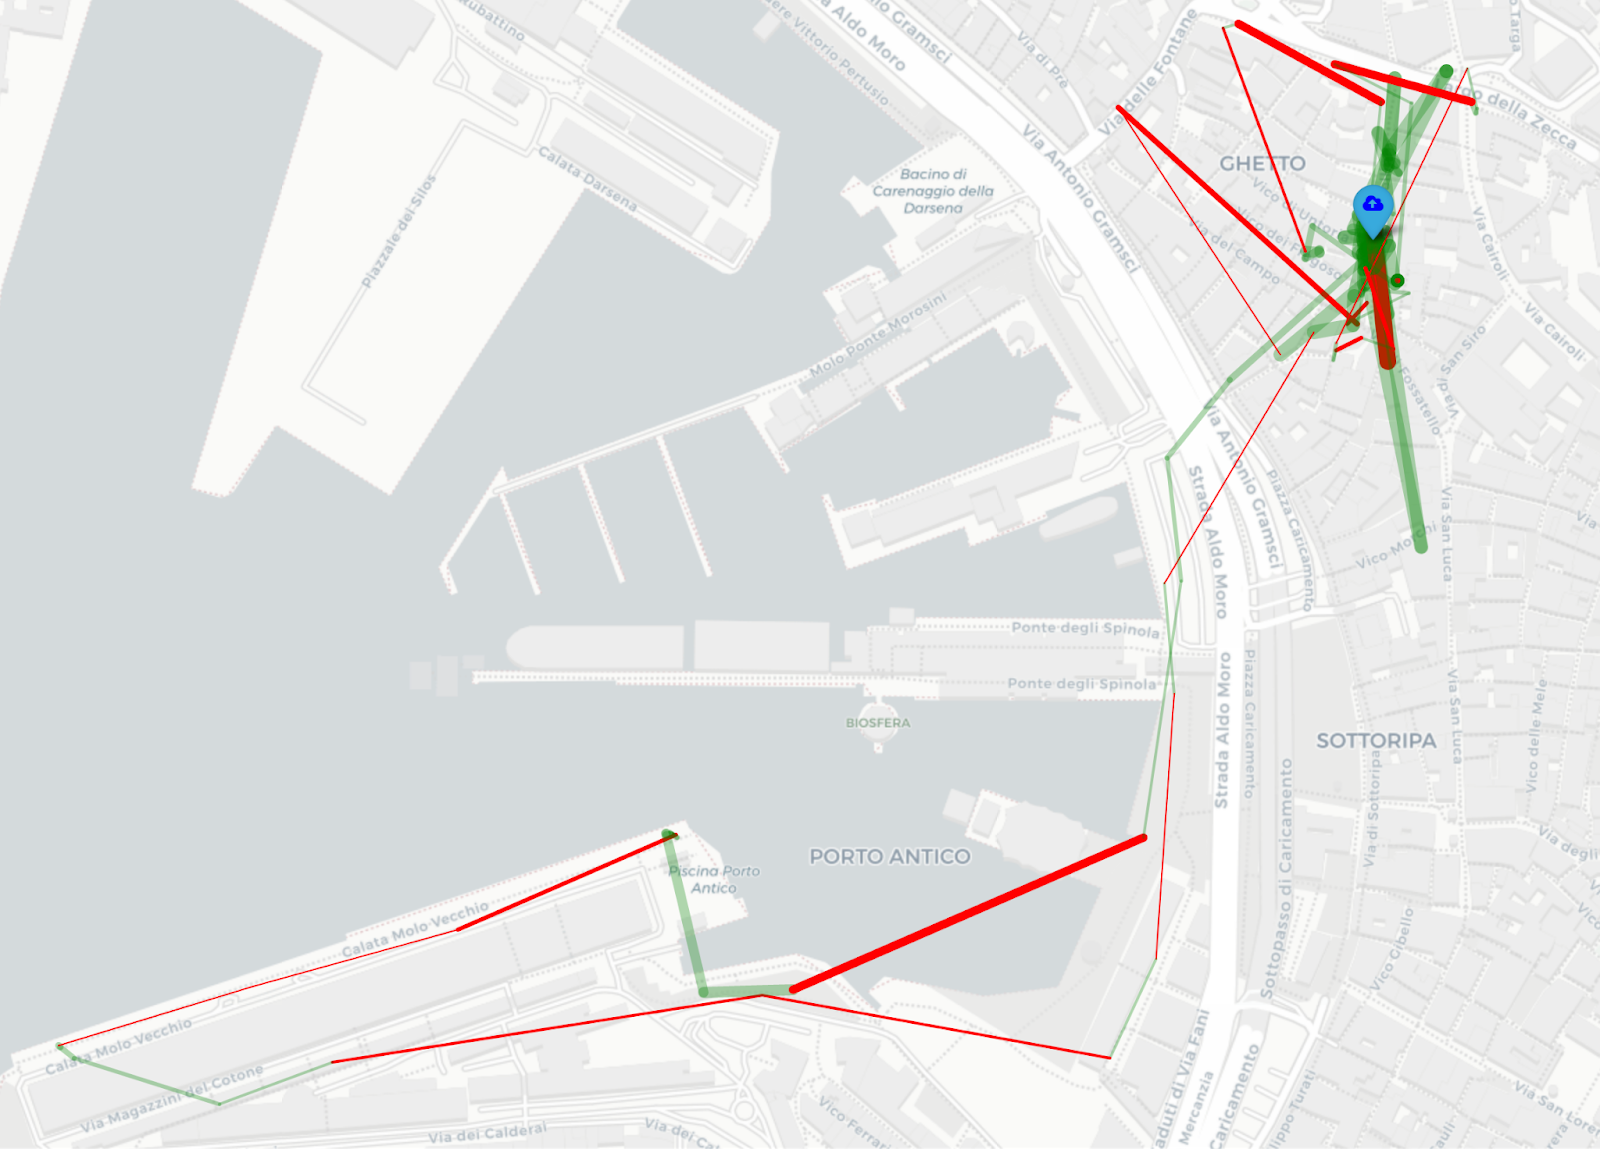
\includegraphics[width=\linewidth]{coloredPath.png}
\caption{Path taken colored by the losses}
\label{chap:conc-colpath}
\end{figure}
In this map the points are connected by lines. A red line between two points indicates that some packets were lost between them. The width of the line indicates the amount of packets lost,  wider lines indicating  bigger losses. 
A green line indicates the opposite, with wider lines indicating the streak of packages received.

Once the points were separated, we analysed the Received signal strength of the points in both 
groups obtaining the figure \vref{chap:conc:rssidist}  comparing both.

\begin{figure}[htpb]
\centering    
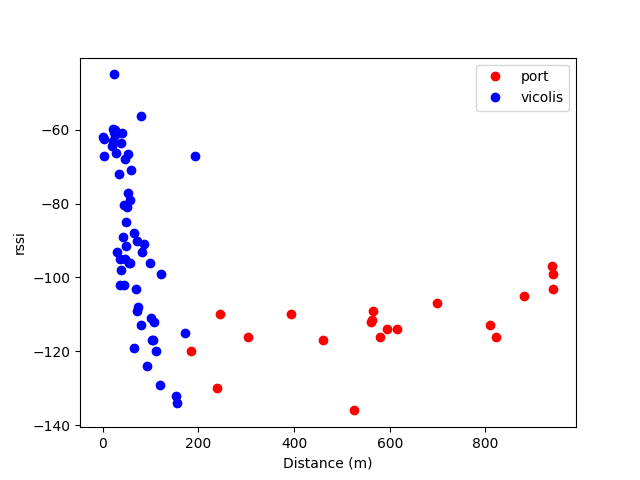
\includegraphics[width=\linewidth]{rssidistancia.png}
\caption{RSSI in function of the distance}
\label{chap:conc:rssidist}
\end{figure}
Here we can clearly see that the signal strength in very dense urban areas decreases very rapidly and fades near the 200 meter distance whereas 
on an open area it maintains stable levels for much longer distances.


Another conclusion can be extracted from this data. If we look at the percentage of packets received when dividing by spreading factor and power
transmitted, on open areas the results closely correlate with theory. On the other hand, the data in the urban dense area highlights that 
these parameters do not have noticeable impact due to the fact that the landscape plays a much more important role.

\begin{figure}[!h]
\centering    
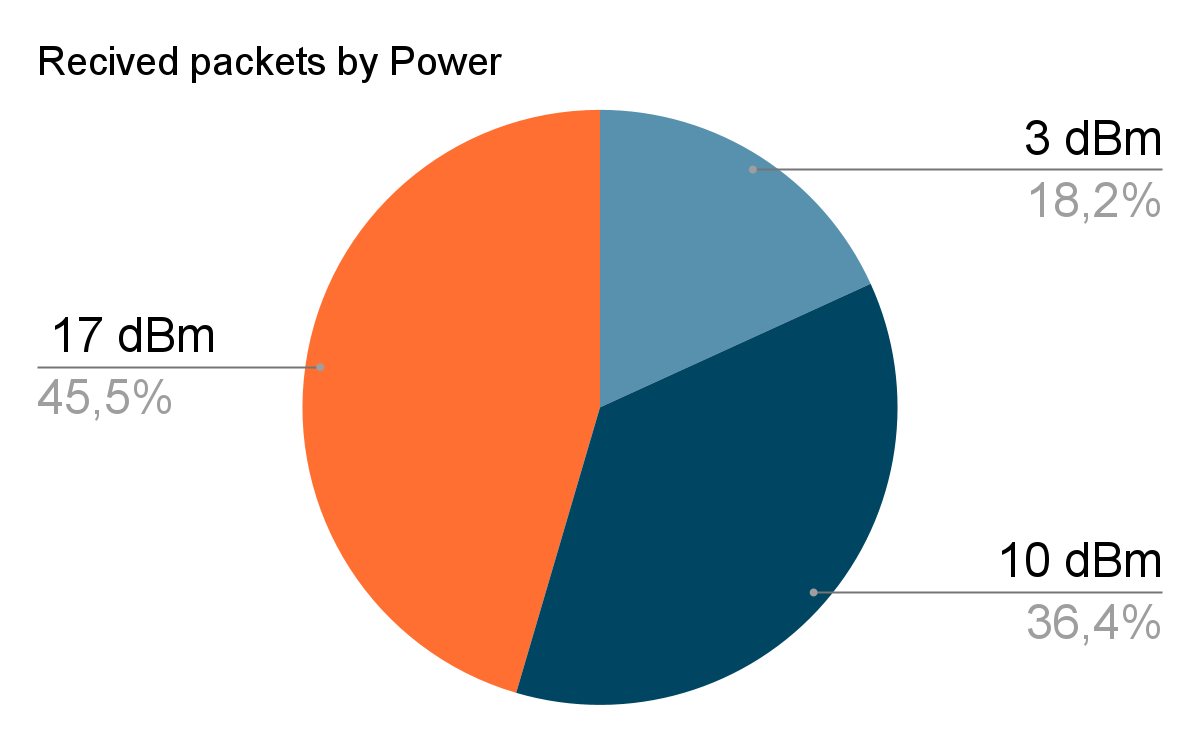
\includegraphics[width=\linewidth]{recivedByPower.png}
\caption{Losses grouped by power}
\label{conc:recivedPow}

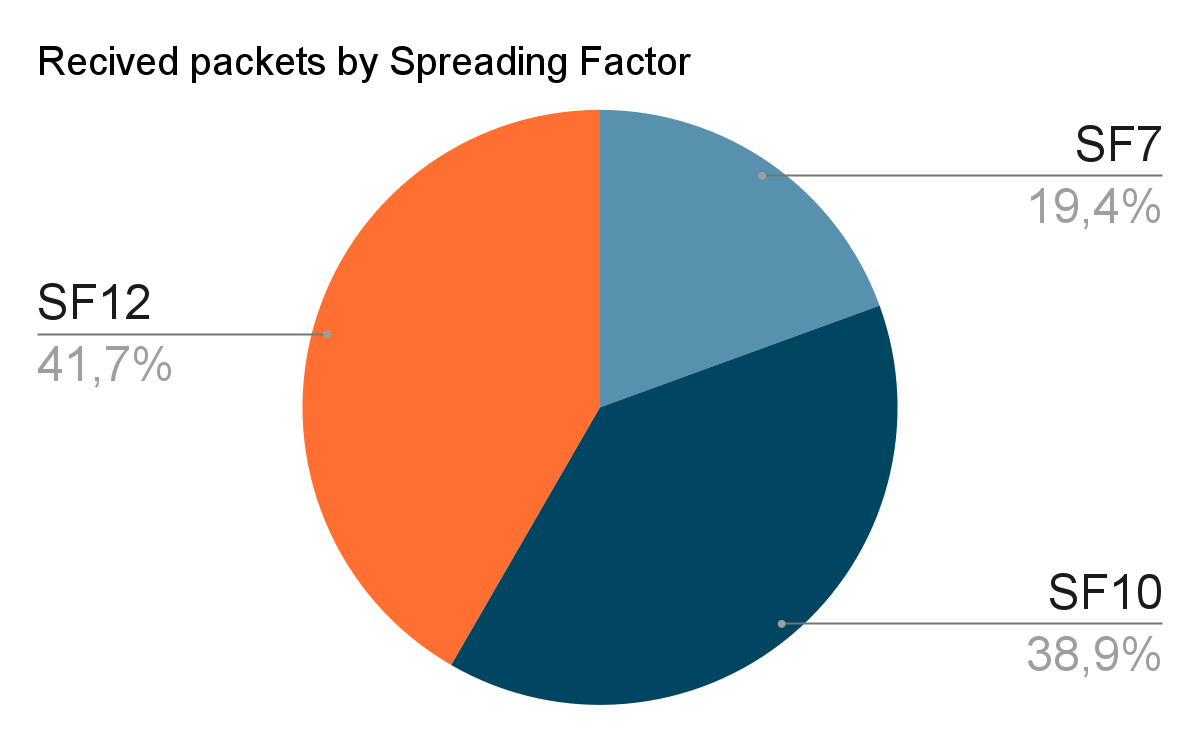
\includegraphics[width=\linewidth]{recivedBySpreading.png}
\caption{Losses gropued by spreading factor}
\label{conc:recivedSp}
\end{figure}
\begin{figure}
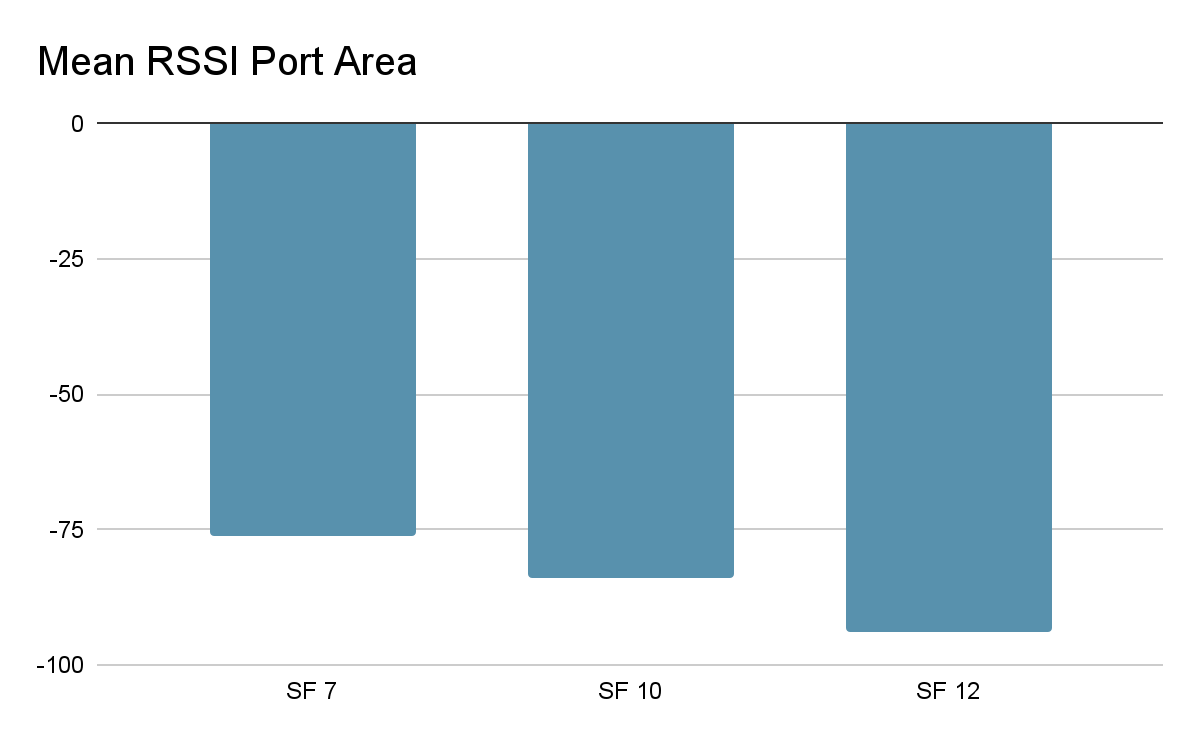
\includegraphics[width=\linewidth]{rssiSpreading.png}
\caption{Mean RSSI grouped by spreading factor}
\label{conc:rssiSp}
\end{figure}

\section{Final conclusions and future work}

The results of the experiments lead to the conclusion that the most important factor when performing a LoRaWan project inside a complex urban area for mobile ED, is the study of the landscape for the different areas. The less obstacles between the ED and the gateway, the better for our communication.
Transmission parameters as the SF or the Tx power are useless when the signal is not received by the gateway because of interference caused by buildings and other obstacles for the signal inside a city. This parameters are relevant for a more open space area, the port area in our case, in which they can make the difference regarding the range for our communication.
The ADR for mobile end nodes where packets are not sent with a high frequency (one per minute) and where the mobile end node is moving with not much speed (walking case) is pointless.
Regarding the future, the limitations due to the duty cycle didn't let us collect the data as we wanted. The transmission interval between packets was controlled by the library used and it was impossible to collect a huge amount of data in a short period of time. Being able to control the time between packets would suppose a great improvement for the experimentation. This improvement would lead to a better analysis of  data regarding the SF and the TX power as more packets would be taken into account and also to build new hypothesis such as how this interval can affect the ADR. 
In order to measure the packet loss depending on distance, a device that collects all the messages the ED is trying to send is needed. By adding this device to the end node, the distance between the ED and the gateway for the packets that doesn't reach the gateway can be calculated. This would suppose a new interesting measure that can be compared depending on the SF and Tx pow in a open space area.




